
\chapter{Grundlagen}
\section{Die OPC Foundation}
Die \ac{opc}-Technologie (OLE for Process Control) wurde entwickelt, um eine interoperable Kommunikation zwischen verschiedenen Plattformen unterschiedlicher Anbieter zu ermöglichen. Bis zum heutigen Zeitpunkt wird sie von über 17 Millionen Anwendungen genutzt \cite{OPCFoundation.15.06.2017}. Im Jahr 2016 wurde \ac{opc} und kann daher von jedem öffentlich auf Github gefunden werden, um die Adoption der Technologie zu erleichtern \cite{OPCFoundation.15.06.2017}.\\

\ac{opc} gilt als besonders sicher und zuverlässig und findet hauptsächlich Anwendung in der industriellen Automatisierung. Die Verantwortung für die Wartung und Entwicklung des Standards liegt bei der \ac{opc} Foundation. Der \ac{opc}-Standard definiert eine Vielzahl von Spezifikationen, die die Schnittstellen zwischen Clients und Servern, sowie zwischen Servern und Servern definieren. Dadurch wird es möglich, Ereignisse und Alarme zu überwachen, Zugriff auf Echtzeit- und historische Daten sowie auf andere Anwendungen zu erhalten.\\

Als \ac{opc} 1996 auf den Markt eingeführt wurde, war es auf speicherprogrammierbare Steuerungen (SPS) ausgelegt und konnte Lese- und Schreibbefehle ausführen. Dadurch war es möglich, Systeme und Produkte nahtlos über \ac{opc} zu kommunizieren \cite{OPCFoundation.15.06.2017}.

\subsection{OPC Unified Architecture}

\ac{opcua} ist ein Kommunikationsprotokoll für industrielle Automatisierungssysteme. Es wurde entwickelt, um eine sichere und zuverlässige Kommunikation zwischen verschiedenen Geräten und Systemen zu ermöglichen. Das Protokoll wurde 2006 eingeführt und hat sich seitdem zu einem weit verbreiteten Standard in der industriellen Automatisierungsbranche entwickelt.\\

\ac{opcua} ist plattformunabhängig und herstellerneutral konzipiert und ermöglicht die Kommunikation zwischen Geräten unterschiedlicher Hersteller. Es bietet eine gemeinsame Sprache für den Datenaustausch zwischen Geräten, was die Integration vereinfacht und das Risiko von Kompatibilitätsproblemen verringert. Darüber hinaus bietet \ac{opcua} eine Reihe erweiterter Funktionen, darunter Echtzeit-Datenzugriff, Ereignisüberwachung und Zugriff auf historische Daten.\\

Einer der Hauptvorteile von \ac{opcua} ist der Fokus auf Sicherheit. Das Protokoll enthält mehrere Sicherheitsfunktionen wie Verschlüsselung und digitale Signaturen, die vor unbefugtem Zugriff und Manipulation schützen. OPC UA verwendet auch ein mehrschichtiges Sicherheitsmodell, das dazu beiträgt, das Risiko von Sicherheitsverletzungen zu mindern.\\

\ac{opcua} ist außerdem skalierbar und flexibel konzipiert, wodurch es für den Einsatz in einer Vielzahl von industriellen Automatisierungsanwendungen geeignet ist. Das Protokoll kann sowohl in lokalen als auch in entfernten Anwendungen verwendet werden und unterstützt sowohl drahtgebundene als auch drahtlose Kommunikation.\\

Zusammenfassend lässt sich sagen, dass \ac{opcua} ein hochentwickeltes Kommunikationsprotokoll ist, das industriellen Automatisierungssystemen eine Reihe von Vorteilen bietet. Sein Fokus auf Sicherheit, Interoperabilität und Skalierbarkeit macht es zu einer idealen Lösung für eine Vielzahl von Anwendungen. Die weit verbreitete Übernahme von \ac{opcua} durch Hersteller und Anwender in der Industrieautomatisierungsbranche bestätigt seinen Wert und Nutzen.\\
\cite{Damm.2009}

\subsection{OPC Sicherheitsvorteile}

\ac{opcua} verfügt über ein großes und skalierbares Sicherheitskonzept, um eine hohe Zugriffsicherheit zu gewährleisten. Falls die Maßnahmen nicht ausreichen, können die Daten auf der Transport-Ebene mittels SSL verschlüsselt werden \cite{Team.06.03.2023}.\\

Um den Sicherheitsanforderungen der Anwendung gerecht zu werden, verfügt OPC UA über den Mechanismus der Endpunkte. Diese haben unterschiedliche Datenstrukturen und Sicherheitseigenschaften. Durch die Vereinheitlichung der Profile (Collaboration Models) können OPC UA-Clients den Inhalt der Daten interpretieren. \\

Für jede Funktion gibt es Profile wie den S95-Standard für die MES-Ankopplung\cite{Team.06.03.2023}. Um die Daten während der Übertragung zu sichern, werden 128- oder 256-Bit-Verschlüsselung, Nachrichtensignierung, Benutzerauthentifizierung und Paketsequenzierung verwendet.\\

OPC UA verwendet außerdem einen Zertifikataustausch, so dass sich jeder Client mittels eines Zertifikats authentifizieren muss. Dadurch wird sichergestellt, dass sich nur Clients mit dem Server verbinden, die auch die Erlaubnis haben \cite{Team.06.03.2023}.

\begin{figure}[htp]
    \centering
    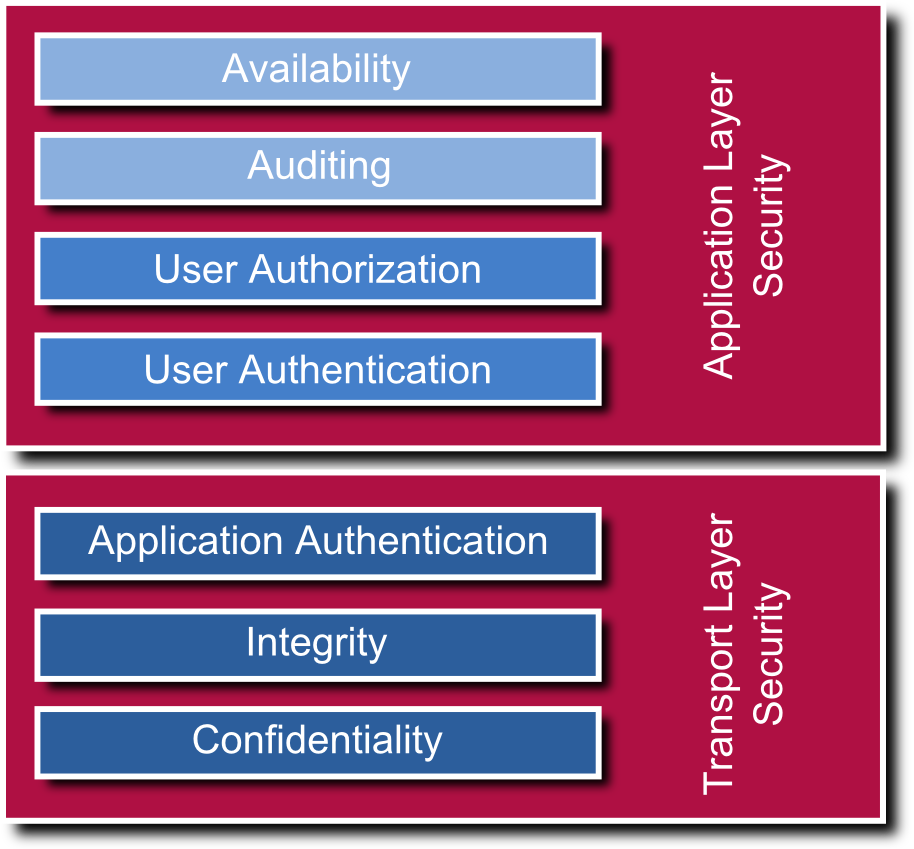
\includegraphics[width=(\textwidth/2)]{Bild/uasecurity.png}
    \caption{UA Sicherheit\cite{Team.06.03.2023}}
    \label{fig:UA Sicherheit}
\end{figure}

\section{Javascript}
JavaScript ist eine hochdynamische, objektorientierte Programmiersprache, die in den 1990er Jahren entwickelt wurde. Ursprünglich als Scriptsprache für Webbrowser konzipiert, wird sie heute in einer Vielzahl von Anwendungsbereichen eingesetzt, einschließlich Webentwicklung, mobilen Anwendungen, Desktop-Software und sogar im Internet der Dinge.\\

JavaScript ist eine interpretierte Sprache, was bedeutet, dass der Quellcode direkt ausgeführt wird, ohne dass er zuvor kompiliert werden muss. Dies ermöglicht es Entwicklern, schnell und einfach Prototypen zu erstellen und Feedback von Benutzern zu erhalten, ohne dass ein Kompilierungsprozess durchgeführt werden muss.\\

Ein wesentliches Merkmal von JavaScript ist seine Fähigkeit, asynchron zu arbeiten. Dies ermöglicht es der Sprache, gleichzeitig mehrere Aufgaben auszuführen, ohne dass die Benutzeroberfläche blockiert wird. Dies ist besonders wichtig bei der Entwicklung von Webanwendungen, da es Benutzern eine bessere Erfahrung ermöglicht, indem sie die Interaktivität und Reaktionszeit verbessert.\\

JavaScript unterstützt eine Vielzahl von Programmierparadigmen, einschließlich objektorientierter, funktionaler und prozeduraler Programmierung. Es bietet eine Fülle von Funktionen, die es Entwicklern ermöglichen, komplexe Anwendungen zu erstellen, einschließlich dynamischer Benutzeroberflächen, Datenbankanbindungen und Netzwerkanwendungen.\\

In Bezug auf die Syntax ähnelt JavaScript C-ähnlichen Sprachen, einschließlich C++ und Java. Es enthält jedoch auch einige einzigartige Funktionen, einschließlich hoher Dynamik und Unterstützung für reguläre Ausdrücke.\\

Zusammenfassend ist JavaScript eine vielseitige, leistungsstarke Programmiersprache, die für eine Vielzahl von Anwendungsbereichen verwendet werden kann. Ihre Fähigkeit, asynchron zu arbeiten, und ihre Unterstützung für mehrere Programmierparadigmen machen sie zu einer attraktiven Wahl für Entwickler.\\
 
\section{Node.js}
Node.js ist eine Open-Source, plattformübergreifende JavaScript-Laufzeitumgebung, mit der Entwickler skalierbare und leistungsstarke Anwendungen erstellen können. Es basiert auf der V8-Engine von Google, die JavaScript in Maschinencode kompiliert, um eine effiziente Ausführung zu ermöglichen. Node.js verwendet ein ereignisgesteuertes, nicht blockierendes E/A-Modell, das es gut geeignet macht, Anwendungen zu erstellen, die eine hohe Durchsatzrate und niedrige Latenzzeiten erfordern.\cite{.06.03.2023}\\

Einer der Schlüsselvorteile von Node.js ist seine Fähigkeit, große Anzahl von gleichzeitigen Verbindungen zu verarbeiten. Im Gegensatz zu herkömmlichen serverseitigen Technologien, die für jede eingehende Verbindung einen neuen Thread oder Prozess erstellen, verwendet Node.js einen einzigen Thread, um alle Verbindungen zu handhaben. Mit diesem Ansatz kann Node.js Tausende von gleichzeitigen Verbindungen verarbeiten, ohne übermäßige Systemressourcen zu verbrauchen.\cite{Node.js.27.02.2023b}\\

Node.js bietet auch ein umfangreiches Ökosystem von Bibliotheken und Modulen, die leicht installiert und in Anwendungen integriert werden können. Dies erleichtert es Entwicklern, komplexe Anwendungen schnell und effizient zu erstellen.\cite{Node.js.27.02.2023}\\

Ein weiterer Vorteil von Node.js ist seine Fähigkeit, auf verschiedenen Plattformen wie Linux, Windows und macOS ausgeführt werden zu können. Diese plattformübergreifende Kompatibilität macht es einfach, Code einmal zu schreiben und auf mehreren Plattformen bereitzustellen.\cite{Node.js.27.02.2023}\\

\section{Typescript}
TypeScript ist eine Programmiersprache, die eine Erweiterung von JavaScript darstellt. Sie bietet optional statisches Typing, was Entwicklern ermöglicht, Fehler vor der Laufzeit zu erkennen, was das Schreiben und die Pflege von komplexem Code erleichtern kann. TypeScript wurde von Microsoft entwickelt und ist heute eine Open-Source-Sprache, die in jedem JavaScript-Projekt verwendet werden kann. TypeScript erweitert JavaScript um Funktionen wie Schnittstellen, Klassen und Typannotationen.\cite{.01.03.2023b}\\

Einer der Vorteile von TypeScript besteht darin, dass es dazu beitragen kann, die Code-Qualität und Wartbarkeit zu verbessern. Durch die Verwendung von statischem Typing können Entwickler Fehler früh im Entwicklungsprozess erkennen, was zu leichter lesbarem Code führen kann. Darüber hinaus bietet TypeScript bessere Werkzeuge und Code-Intelligenz, was es einfacher macht, mit großen Code-Basen zu arbeiten und mit anderen Entwicklern zusammenzuarbeiten.\cite{.06.03.2023b}\\

TypeScript ist auch kompatibel mit beliebten JavaScript-Bibliotheken und Frameworks, was es einfach macht, in vorhandene Projekte zu integrieren. Es kann für Front-End-Entwicklung mit Frameworks wie Angular, React und Vue.js sowie für Back-End-Entwicklung mit Node.js verwendet werden.\cite{Udemy.06.03.2023}\\

Zusammenfassend ist TypeScript eine leistungsfähige Sprache, die dazu beitragen kann, die Code-Qualität und Wartbarkeit zu verbessern. Seine Kompatibilität mit beliebten JavaScript-Bibliotheken und Frameworks sowie seine umfangreichen Werkzeuge und Code-Intelligenz machen es zu einer beliebten Wahl unter Entwicklern. Entwickler können Ressourcen wie die offizielle TypeScript-Website, die TypeScript-Dokumentation und TypeScript-Tutorials von Udemy finden, um mit TypeScript zu beginnen.\cite{.01.03.2023}\\

\section{Der SICK RFU6 und seine Ensatzgebiete}

Der RFU ist eine intelligente Identifikationslösung von SICK AG und basiert auf der \ac{rfid}-Technologie, die für Radio Frequency Identification steht. Durch den Einsatz von Funkwellen ist es möglich, Objekte automatisch zu identifizieren. Ein \ac{rfid}-Transponder, der an dem Objekt angebracht ist, wird vom RFU erkannt und die darauf gespeicherten Daten ausgelesen. Es gibt drei verschiedene Arten von \ac{rfid}-Transpondern. Passive Transponder nutzen die Energie des elektromagnetischen Feldes des \ac{rfid}-Readers, um Daten zu senden und zu empfangen. Semi-passive und aktive Transponder haben zusätzlich eine Batterie, die eine höhere Reichweite ermöglicht und es ihnen ermöglicht, Daten wie Temperatur oder Feuchtigkeit zu erfassen und zu speichern.\cite{.07.03.2023}\\

Die Größe des SICK \ac{rfid}-Readers variiert und beeinflusst vor allem die Lese-Reichweite. Der RFU ist in der Lage, auch verschmutzte und verdeckte Objekte zu erkennen, da keine Sichtverbindung zum Transponder erforderlich ist. Die \ac{rfid}-Technologie gilt allgemein als sehr fehlerverzeihend und flexibel, da weder eine exakte Laserlinie noch eine bestimmte Schärfentiefe beachtet werden muss. Die Identifikation großer Objekte mit undefinierter Transponderposition ist durch hohe Leseabstände kein Problem. Die Datenübertragung ist verschlüsselt, was eine hohe Fälschungssicherheit und Datenschutz gewährleistet.\cite{.07.03.2023}\\

\ac{rfid}-Reader sind in der Industrie sehr vielseitig einsetzbar. Sie werden oft für die Werkstückidentifikation in der Prozessautomation oder für die Rückverfolgung von Transportbehältern in der Logistik eingesetzt. Sie eignen sich auch für die Überwachung des Warenein- und -ausgangs in der Logistik oder zur Identifikation von Zügen und Waggons im Schienenverkehr sowie zur elektronischen Mauterfassung.\cite{.07.03.2023}\\
\cite{.07.03.2023}

\begin{figure}[H]
    \centering
    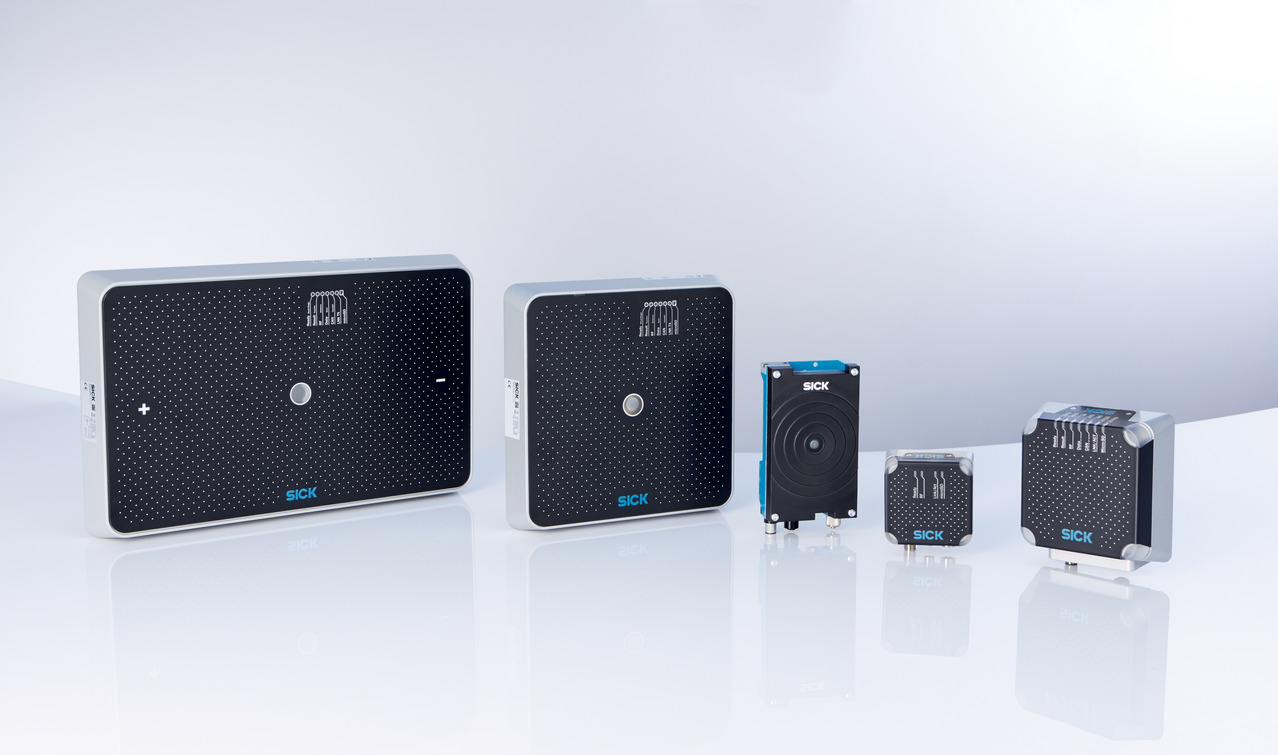
\includegraphics[width=(\textwidth/2)]{Bild/RFU.jpg}
    \caption{RFU\cite{.17.08.2021}}
    \label{fig:RFU}
\end{figure}


\section{UAExpert}
Der UaExpert ist ein OPC UA Testclient, der als universeller OPC UA Testclient entwickelt wurde und Funktionen wie DataAccess, Alarms \& Conditions, HistoricalAccess und den Aufruf von OPC UA Methoden unterstützt. Der Testclient wurde in C++ programmiert und ist plattformunabhängig. Die Benutzeroberfläche wurde mit der GUI-Bibliothek Qt erstellt und kann durch zusätzliche Plugins erweitert werden.\\

Das Basissystem des UaExpert umfasst grundlegende Funktionen wie Zertifikatsmechanismen, Discovery Service, Verbindungsherstellung, Browsing des Informationsmodells und das Lesen von Attributen und Referenzen von OPC UA Knoten. Die Projektansicht zeigt die OPC UA Server und die Adressraum-Ansicht stellt das Informationsmodell des OPC UA Servers in einer Baumstruktur dar. Die Ansichten der Dokument-Plugins befinden sich im Zentrum des Fensters, einschließlich der OPC UA DataAccess View, die Variablen beobachtet und Werte, Zeitstempel und den Status einzelner Knoten anzeigt. Weitere Ansichten können mit dem "Add Document" -Button hinzugefügt werden.\\
\section{Wireshark}
Wireshark ist ein Open-Source-Netzwerkprotokoll-Analyzer, der verwendet wird, um Netzwerkverkehr aufzufangen, zu analysieren und zu visualisieren. Mit Wireshark können Benutzer den gesamten Datenverkehr auf einem Netzwerk überwachen und analysieren, einschließlich der Informationen, die zwischen verschiedenen Geräten und Anwendungen ausgetauscht werden. Es ermöglicht Benutzern, den Datenverkehr in Echtzeit oder aus zuvor aufgezeichneten Daten zu analysieren und Probleme in der Netzwerkkommunikation zu identifizieren und zu beheben.




